\section{Theoretical Background} \label{theory}

This chapter deals with the past and present research in the relevant area which include literature review. This includes 
the significance of precise modelling of the ship's speed and its subsequent use in forecasting the ship's operation.
The theoretical background of Random Forest Regression will be discussed in this chapter. 

\subsection{Literature Review}\label{litreview}

The work by Yan et al. \cite{Yan.2021} provides a thorough review of the different attempts that have been made by different authors  to predict different parameters of ship's operation, this includes ship's fuel consumption. Per definition by Haranen et al. \cite{MichaelHaranen.2016}, the modelling of ship operation is categorised into White Box Model (WBM), Black Box Model (BBM) and Grey Box Model (GBM). Machine learning approach is categorised as BBM, BBM approach is defined as purely data driven approach requiring no prior knowledge about the ship operation. The literature review by Yan et al. \cite{Yan.2021} indicated that about $42\%$ of the research utilised BBM model based on machine learning approach.\\ 

Majority of the BBM approach based on ML is dominated by ANN \cite{Yan.2021}. However, there are literatures that considered decision tree-based modelling approach to predict fuel consumption. Some example of decision tree based modelling include Decision Tree (DT), Random Forest (RF) and Extra Tree (ET). Soner et al. \cite{Soner.2018} implemented tree-based model, which include bagging, random forest (RF), and bootstrap. In their work, they used data captured from onboard sensors of a ferry to predict speed through water and fuel consumption per hour. From the test dataset, the random forest model described root mean square error (RMSE) of $0.34$ Knots during its prediction of Speed Through Water (STW). Yan et al. \cite{Yan.2020} used random forest (RF) model to minimise fuel consumption for a voyage of a dry bulk ship. The model use ship operational data and sea and weather data from noon report and EMCWF. The prediction performance report from this literature reported mean absolute percentage error (MAPE) of $7.91\%$.\\      

The research by Gkerekos et al. \cite{Gkerekos.2019} highlighted the performance of different machine learning models to predict ship's fuel consumption per day using both noon data and automated data logging and monitoring (ADLM) system from a bulk carrier. This research concludes that tree based model displayed good prediction performance on both noon data and sensor based data. Using default parameters, RF model obtained $R^2$ score of $87.55\%$ and $96.26\%$ for noon-data datasets and sensor-based data respectively. It is also noted that it that the data from a 3-month period in ADLM system would be sufficient to create a model with better performance than the model generated by noon data from a collection period of 2.5 year. This literature also concluded that automatic sensor-based data have the potential to increase the model accuracy score, $R^2$, by $5-7\%$ across different machine learning models.\\
\newpage

Li et al. \cite{Li.2022} performed more extensive research on the effects of data fusions between meteorological data, ship voyage data and AIS data on different machine learning models to predict the ship's FOC. This research highlighted the advantage of fusing meteorological data and ship voyage data. The evaluation on different model performance indicated that RF are among preferable model candidate that could be used in commercial scale due to its good prediction capability and robustness against different datasets. The findings in this research reported that $R^2$ score are above $96\%$ when deployed on the best datasets and achieved $R^2$ score in range between $74\% - 90\%$ over test data. This literature also exhibited the robustness of RF, as it attained the lowest standard deviation at $0.015$ of the $R^2$ score when evaluated against random splits of datasets.\\

Abebe et al. \cite{Abebe.2020} used different approach in their research by predicting the ship's Speed Over Ground (SOG) instead of FOC. In this work, AIS data and noon-report weather data from 14 tracks and 62 ships are used for the SOG prediction. The observation showed that RF model achieved RMSE of $0.25$ knots, while using $489$ seconds for training. Decision tree achieved RMSE of $0.36$ knots, taking up $52$ seconds for training. This shows that RFR outperforms DTR at cost of computational power.\\

This literature review described the capability of Random Forest Regressor to predict fuel consumptions and ship speed, irrespective of data source and type of data used. Promising results from different performance measures across different literatures indicated the capability random forest model as predictor. As such, this thesis aims to find optimisation possibilities to extract maximum prediction performance from random forest. Due to the nonlinear, third order function estimate of fuel consumption \cite{Ronen.1982,Ronen.2011}. Accurate prediction of ship speed is paramount to ensure optimal ship operation resulting in increase of profitability. 

\subsection{Decision Tree}\label{dt_theo}

Decision tree is a non-parametric model that is able to perform both classification and regression tasks for discrete variable and continuous variable respectively. It is a powerful algorithm, capable of fitting complex datasets. The model requires very little to no data preprocessing \cite{Geron.2019,Hastie.2009}. Decision tree is a white box model\footnote{This is not to be confused with the definition described by Haranen et al. \cite{MichaelHaranen.2016} regarding modelling of ship operation.} \cite{Geron.2019}. In machine learning sense, this means that the model is intuitive and the structure of the model is interpretable. Thus, the structure of the model can be analysed in detail. To understand the principle of random forest, understanding how decision tree operates is necessary as the principle working of random forest stems from decision trees \cite{Geron.2019,Affenzeller.2020}. In this thesis, We shall only discuss the underlying principle of regression tree.\\  
\newpage

To train Decision Trees. {\tt Scikit-Learn} \cite{FabianPedregosa.2011} uses the \emph{Classification and Regression Tree} (CART) algorithm. Partition space shown by figure \ref{fig:partitionspace} are used to illustrate the decision of CART algorithm. This process can be alternatively represented by the binary tree of figure \ref{fig:partitiontree}, observation that satisfies the condition are assigned to the left branch and the opposite is assigned to the right branch. Here, we can see the interpretability of a tree based model. The partition space can be represented by a single tree, this is especially helpful when multiple input variables are involved, the inputs can be represented by a single tree \cite{Hastie.2009}.

\begin{figure}[h]
\centering
\begin{minipage}[b]{.5\textwidth}
    \centering
    \begin{tikzpicture}[x=0.75pt,y=0.75pt,yscale=-1,xscale=1]
    %uncomment if require: \path (0,433); %set diagram left start at 0, and has height of 433
    
    %Shape: Square [id:dp5731268858272198] 
    \draw   (180,110) -- (370,110) -- (370,300) -- (180,300) -- cycle ;
    %Straight Lines [id:da615072570759449] 
    \draw    (250,110) -- (250,300) ;
    %Straight Lines [id:da8002566967918264] 
    \draw    (300,110) -- (300,300) ;
    %Straight Lines [id:da4409034763483005] 
    \draw    (180,230) -- (250,230) ;
    %Straight Lines [id:da07514682530914596] 
    \draw    (300,170) -- (370,170) ;
    
    % Text Node
    \draw (131,192.4) node [anchor=north west][inner sep=0.75pt]    {$X_{2}$};
    % Text Node
    \draw (261,340.4) node [anchor=north west][inner sep=0.75pt]    {$X_{1}$};
    % Text Node
    \draw (157,222.4) node [anchor=north west][inner sep=0.75pt]    {$t_{2}$};
    % Text Node
    \draw (201,252.4) node [anchor=north west][inner sep=0.75pt]    {$R_{1}$};
    % Text Node
    \draw (201,162.4) node [anchor=north west][inner sep=0.75pt]    {$R_{2}$};
    % Text Node
    \draw (268,192.4) node [anchor=north west][inner sep=0.75pt]    {$R_{3}$};
    % Text Node
    \draw (321,132.4) node [anchor=north west][inner sep=0.75pt]    {$R_{4}$};
    % Text Node
    \draw (321,220.4) node [anchor=north west][inner sep=0.75pt]    {$R_{5}$};
    % Text Node
    \draw (241,310.4) node [anchor=north west][inner sep=0.75pt]    {$t_{1}$};
    % Text Node
    \draw (291,312.4) node [anchor=north west][inner sep=0.75pt]    {$t_{3}$};
    % Text Node
    \draw (381,162.4) node [anchor=north west][inner sep=0.75pt]    {$t_{4}$};
    
    \end{tikzpicture}
    
    \captionof{figure}{Example of partition space} 
    \label{fig:partitionspace}
\end{minipage}%
\begin{minipage}[b]{.5\textwidth}
    \centering
    \begin{tikzpicture}
        \tikzset{level distance=65pt,sibling distance=10pt,edge from parent/.style=
        {draw,edge from parent path={(\tikzparentnode.south)
                                -- +(0,-8pt)
                                -| (\tikzchildnode)}}}
    \Tree [.$X_1\leq t_1$ [.$X_2\leq t_2$ [.$R_1$ ] [.$R_2$ ] ]
        [.$X_1\leq t_3$ [.$R_3$ ]
        [.$X_2\leq t_4$ [.$R_4$ ] [.$R_5$ ] ] ] ]
    \end{tikzpicture}
    \captionof{figure}{Example of partition tree} 
    \label{fig:partitiontree}
\end{minipage}
\end{figure}

Now, we need to understand the principle of selection for the feature $X_t$ and threshold $t_k$. We shall first start with the principle of selection of the threshold $t_k$. Assuming a case with single feature $X$ and response $Y$, with $m$ data points. The following steps are observed: 
\begin{enumerate}
    \item Possible thresholds are determined by calculating the splitting value (For example, suppose there are data points at $X = [0.2,0.4]$, then the splitting value is the value in between i.e. $t_k = 0.3$)
    \item Calculate the mean of data points of the left and right partition space respectively, Defined by the following equation $\hat{y}_{node} = \frac{1}{m_{node}}\sum\limits_{i\in node} y ^ {(i)}$
    \item Calculate the mean squared error (MSE) of each data points in its respective partition space. Through the equation $MSE_{node} = \sum\limits_{i\in node}(\hat{y}_{node} - y^{(i)} )^2$ 
    \item The MSE from the respective partition space is summed.
    \item Step $1 - 4$ is recursively repeated, until the minimum of the cost function $J(X,T_k)$, i.e. minimum MSE, is determined:
     \begin{equation}\label{costfun}
        J(X,T_k) = \frac{m_{left}}{m}MSE_{left} + \frac{m_{right}}{m}MSE_{right}
        \begin{cases}
            MSE_{node} = \sum\limits_{i\in node}(\hat{y}_{node} - y^{(i)} )^2 \\
            \hat{y}_{node} = \frac{1}{m_{node}}\sum\limits_{i\in node} y ^ {(i)}
        \end{cases}   
    \end{equation}
\end{enumerate} 

Once complete, then the regions is further split into two more regions and this process is recursively continued until a stopping rule is applied. The stopping rule are either when the tree reaches the maximum depth, (This is controlled by the parameter {\tt max\_depth} in {\tt Scikit-Learn}), or when it cannot find a split that can further reduce MSE. This best split also corresponds to the best possible fit to the predicted value. Same principle is also applied when multiple feature is present. Consider there are $X_t$ features, then for each respective features $X_1,X_2,\dots,X_t$, The MSE for each of the features is calculated using the cost function $J(X,T_k)$. The feature that can \emph{\textbf{minimise}} the cost function will be selected as the root of the tree. The tree is then grown further by recursively repeating this process \cite{Hastie.2009,Geron.2019}.\\

While powerful, decision tree unfortunately suffer from overfitting when the model is unconstrained. Decision tree makes very few assumptions regarding the training data. Therefore, it will adapt to the training data and fitting it very closely. Therefore it is necessary to regularise i.e. restrict the decision tree's freedom during the training. By tuning the maximum tree depth through {\tt max\_depth} parameter, this could potentially help reduce overfitting. Additionally, setting the amount of minimum number of samples a leaf node have through {\tt min\_samples\_leaf} can alleviate overfitting as well.  







\begin{tikzpicture}[x=0.75pt,y=0.75pt,yscale=-1,xscale=1]
    %uncomment if require: \path (0,452); %set diagram left start at 0, and has height of 452
    
    %Shape: Axis 2D [id:dp697661158302031] 
    \draw  (220,297.8) -- (517.5,297.8)(249.75,80) -- (249.75,322) (510.5,292.8) -- (517.5,297.8) -- (510.5,302.8) (244.75,87) -- (249.75,80) -- (254.75,87)  ;
    %Image [id:dp23308396965327827] 
    \draw (245,305) node [rotate=-40.58] {\includegraphics[width=26.87pt,height=72.39pt]{02_figures/ferry.jpg}};
    
    
    
    
\end{tikzpicture}




\subsection{Ship speed}


\subsection{Modelling}




